\documentclass[../main.tex]{subfiles} 
\usepackage{ctex}
\usepackage{xltxtra}
\usepackage{graphicx}
\usepackage{booktabs}
\usepackage{amsmath}
\usepackage{mathdots}
\usepackage{amssymb}
\usepackage{cite}
\usepackage{appendix}
\usepackage{array}
\usepackage{subfigure}
\begin{document}

    \subsection{评价方法}

        绘制混淆矩阵,根据混淆矩阵的结果得出四个评价指标:Accuracy、Precision、Recall、F1-Score;

        使用10折交叉验证,在每次交叉验证的时候记录该次训练的混淆矩阵以及四个评价指标,最后训练结束后对10次结果取平均值并进行混淆矩阵的绘制和评价指标的输出。
        
        利用sklearn.metrics.plot\_roc\_curve绘制模型的ROC曲线,得到AUC值;

        利用sklearn.model\_selection.learning\_curve根据训练样本的数量绘制模型的学习曲线。

    \subsection{SVC}

        混淆矩阵如图34.(a)所示,ROC曲线如图34.(b)所示,Accuracy、Precision、Recall、F1-Score如图34.(c)所示,drop部分特征前学习曲线如图34.(d)所示,drop部分特征后学习曲线如图34.(e)所示。

        \begin{figure}[H]
            \centering
            \subfigure[混淆矩阵]
            {
                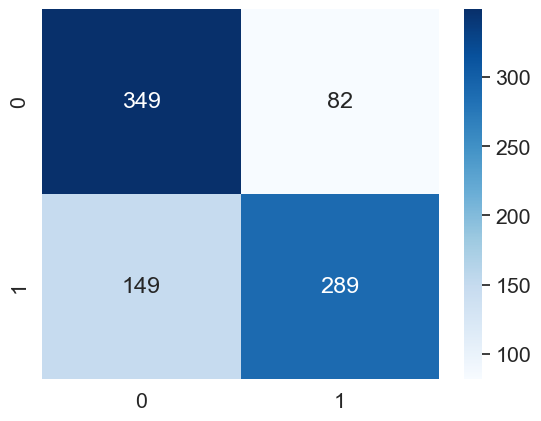
\includegraphics[scale=0.2]{Sec7_1.png}
            }
            \subfigure[ROC曲线]
            {
                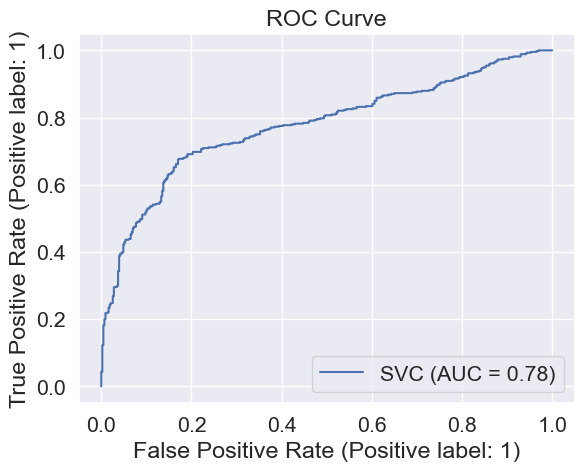
\includegraphics[scale=0.2]{Sec7_3.png}
            }

            \subfigure[Accuracy、Precision、Recall、F1-Score]
            {
                
\includegraphics[scale=0.3]{Sec7_2.png}
            }

            \subfigure[drop部分特征前学习曲线]
            {
                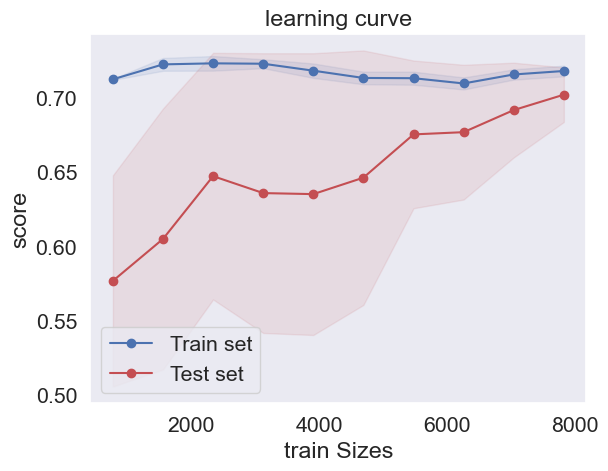
\includegraphics[scale=0.2]{Sec7_4.png}
            }
            \subfigure[drop部分特征后学习曲线]
            {
                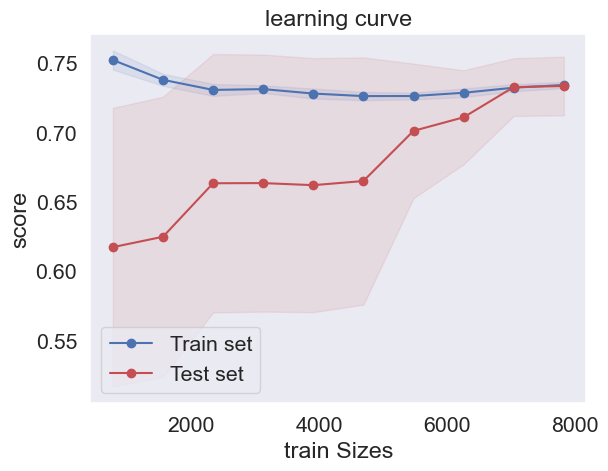
\includegraphics[scale=0.2]{Sec7_26.png}
            }
            \caption{SVC}
        \end{figure}

        从图中的混淆矩阵和四个评价指标可以看出,模型的效果并不好,很容易产生错分类的情况,并且由于数据量较大,SVM的训练时间长于其他模型,计算量较大。
        并且将正类样本错分为负类样本的数量比将负类样本错分为正类样本的数量多,可以看出模型对于正类样本的学习较差。

        经过思考,我认为模型效果较差的原因为缺失值填补的问题,因为SVM本身是对于缺失值较为敏感的模型,而该数据集缺失值较多,填补过程中使用了很多相关性信息进行填补,可能导致模型效果较差。

    \subsection{Decision Tree}

    混淆矩阵如图35.(a)所示,ROC曲线如图35.(b)所示,Accuracy、Precision、Recall、F1-Score如图35.(c)所示,drop部分特征前学习曲线如图35.(d)所示,drop部分特征后学习曲线如图35.(e)所示。

        \begin{figure}[H]
            \centering
            \subfigure[混淆矩阵]
            {
                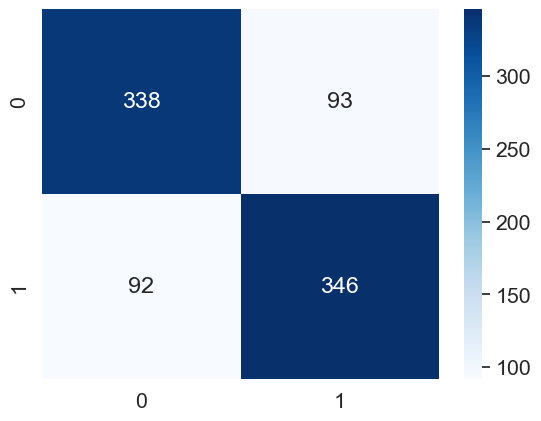
\includegraphics[scale=0.2]{Sec7_5.png}
            }
            \subfigure[ROC曲线]
            {
                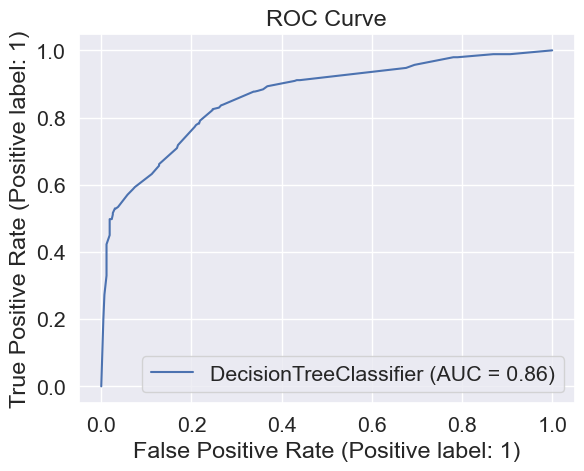
\includegraphics[scale=0.2]{Sec7_7.png}
            }

            \subfigure[Accuracy、Precision、Recall、F1-Score]
            {
                
\includegraphics[scale=0.3]{Sec7_6.png}
            }

            \subfigure[drop部分特征前学习曲线]
            {
                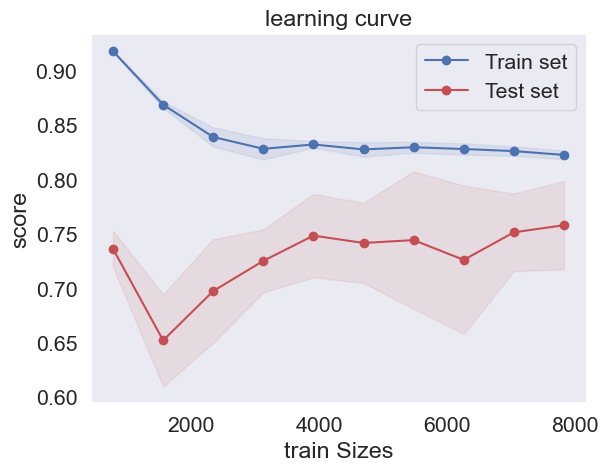
\includegraphics[scale=0.2]{Sec7_8.png}
            }
            \subfigure[drop部分特征后学习曲线]
            {
                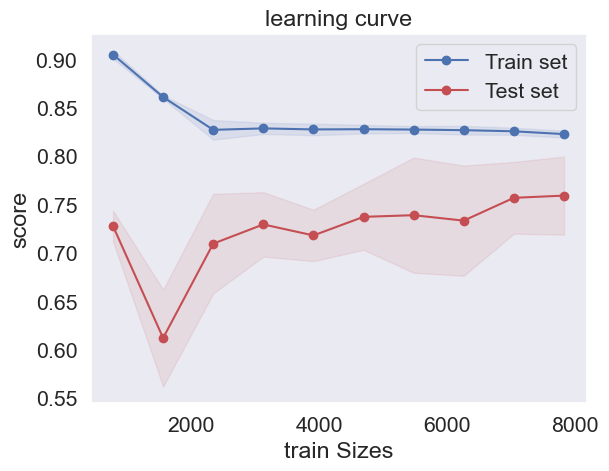
\includegraphics[scale=0.2]{Sec7_27.png}
            }
            \caption{Decision Tree}
        \end{figure}

        可以发现,决策树模型的效果比起SVM提高了接近10\%。从混淆矩阵中可以发现FP和FN的数量是相同的,相比起来SVM模型训练结果FN错分的数量比起FP大得多,并且都比决策树模型多。可以看出决策树模型在提升了对于负类样本的学习的同时更显著提高了对于正类样本的学习能力。

        我认为是因为一方面决策树相比起SVM对缺失值不敏感,并且可以处理不相关特征数据。但是从学习曲线可以发现模型在2000个样本的时候得分有个突降,并且模型不收敛,属于是高方差的情况,并且泛化能力很差,可能是因为模型数据特征过多导致。

    \subsection{Naive Bayes}

        混淆矩阵如图36.(a)所示,ROC曲线如图36.(b)所示,Accuracy、Precision、Recall、F1-Score如图36.(c)所示,drop部分特征前学习曲线如图36.(d)所示,drop部分特征后学习曲线如图36.(e)所示。

        \begin{figure}[H]
            \centering
            \subfigure[混淆矩阵]
            {
                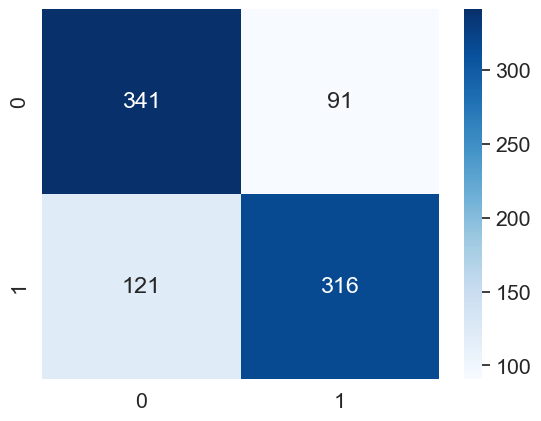
\includegraphics[scale=0.2]{Sec7_9.png}
            }
            \subfigure[ROC曲线]
            {
                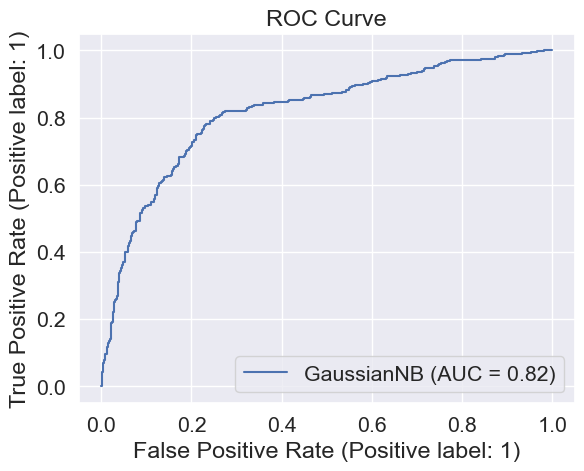
\includegraphics[scale=0.2]{Sec7_11.png}
            }

            \subfigure[Accuracy、Precision、Recall、F1-Score]
            {
                
\includegraphics[scale=0.3]{Sec7_10.png}
            }

            \subfigure[drop部分特征前学习曲线]
            {
                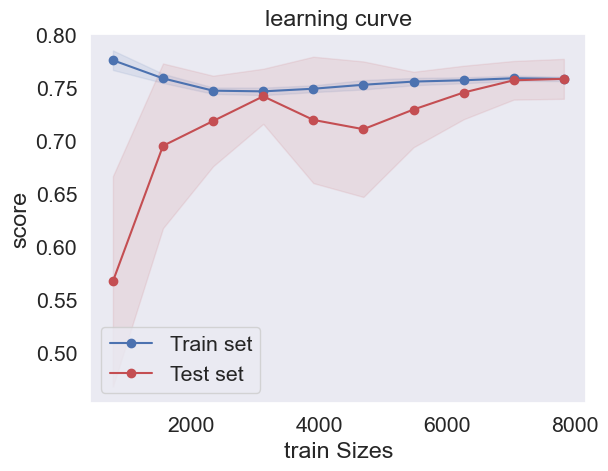
\includegraphics[scale=0.2]{Sec7_12.png}
            }
            \subfigure[drop部分特征后学习曲线]
            {
                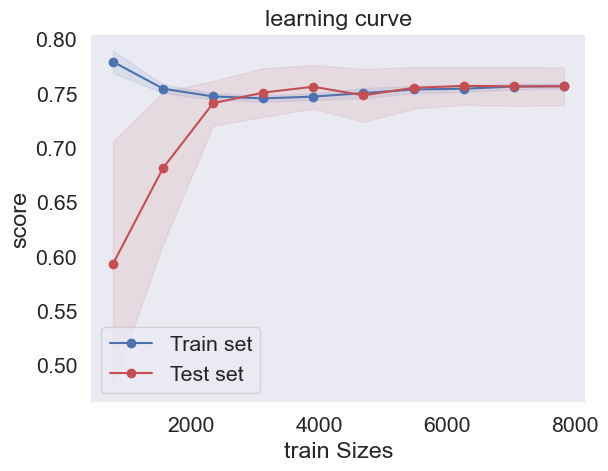
\includegraphics[scale=0.2]{Sec7_30.png}
            }
            \caption{Naive Bayes}
        \end{figure}

        一开始使用的是MultinomialNB模型,模型的精度只有接近65\%,效果非常差,可能是因为模型中有部分特征是较为连续化的数据,而多项式贝叶斯模型主要处理的是离散型数据,因此效果较差。
        换用GaussianNB模型后,可以发现训练效果得到了很好的改善,并且通过观察训练集和测试集学习曲线可以发现曲线收敛效果较好,但得分较差。说明模型对已知数据和未知数据都不能进行准确的预测,属于高偏差。这种情况模型很可能是欠拟合。
        但是在drop掉部分特征后学习曲线出现了交叉,说明模型的拟合出现了问题,该问题未得到很好的解决。

    \subsection{KNN}

        混淆矩阵如图37.(a)所示,ROC曲线如图37.(b)所示,Accuracy、Precision、Recall、F1-Score如图37.(c)所示,drop部分特征前学习曲线如图37.(d)所示,drop部分特征后学习曲线如图37.(e)所示。

        \begin{figure}[H]
            \centering
            \subfigure[混淆矩阵]
            {
                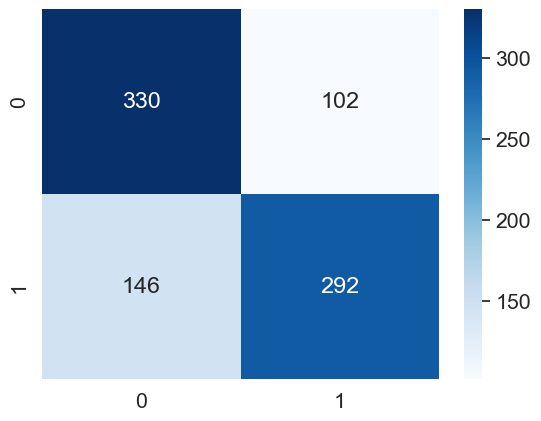
\includegraphics[scale=0.2]{Sec7_13.png}
            }
            \subfigure[ROC曲线]
            {
                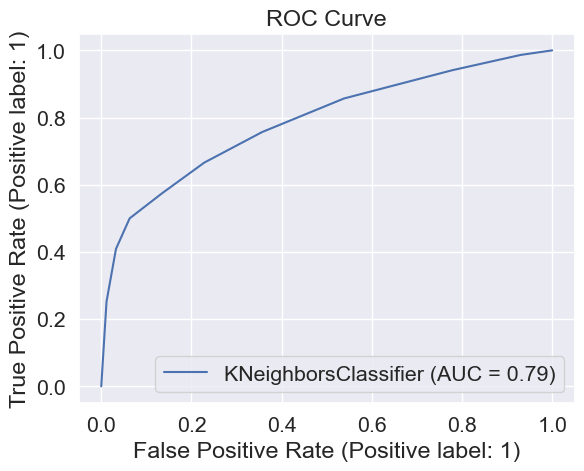
\includegraphics[scale=0.2]{Sec7_15.png}
            }

            \subfigure[Accuracy、Precision、Recall、F1-Score]
            {
                
\includegraphics[scale=0.3]{Sec7_14.png}
            }

            \subfigure[drop部分特征前学习曲线]
            {
                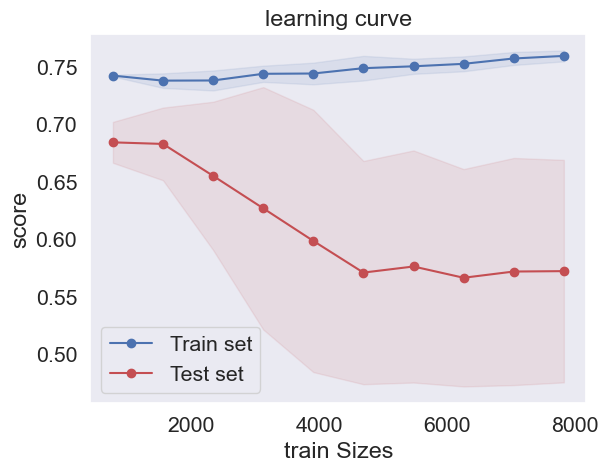
\includegraphics[scale=0.2]{Sec7_16.png}
            }
            \subfigure[drop部分特征后学习曲线]
            {
                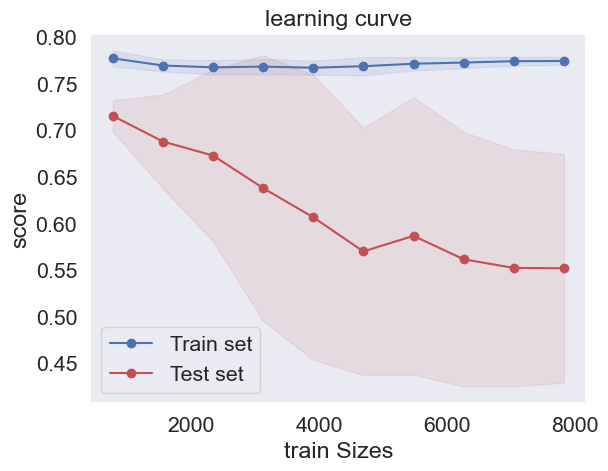
\includegraphics[scale=0.2]{Sec7_25.png}
            }
            \caption{KNN}
        \end{figure}

        可以发现KNN的效果甚至没有SVM好,观察学习曲线可以发现,对于测试集的score在2000个样本后出现了大幅度下滑,一方面数据量极大,并且维度较高,没有经过降维处理,样本数据在样本空间的分布可能较为复杂,导致模型在寻找邻居的时候出现问题,第二个方面使用的邻居数量相比起样本数量少的多。

    \subsection{Random Forest}

        混淆矩阵如图38.(a)所示,ROC曲线如图38.(b)所示,Accuracy、Precision、Recall、F1-Score如图38.(c)所示,drop部分特征前学习曲线如图38.(d)所示,drop部分特征后学习曲线如图38.(e)所示。

        \begin{figure}[H]
            \centering
            \subfigure[混淆矩阵]
            {
                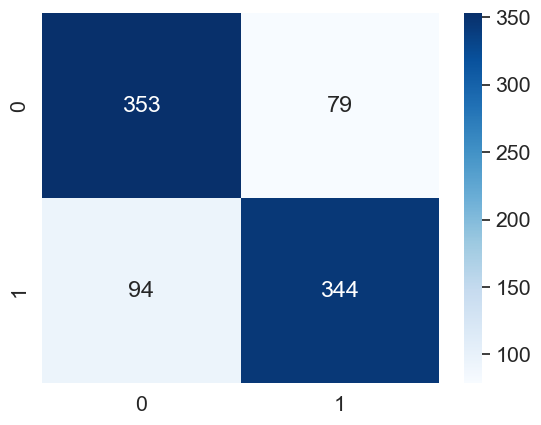
\includegraphics[scale=0.2]{Sec7_17.png}
            }
            \subfigure[ROC曲线]
            {
                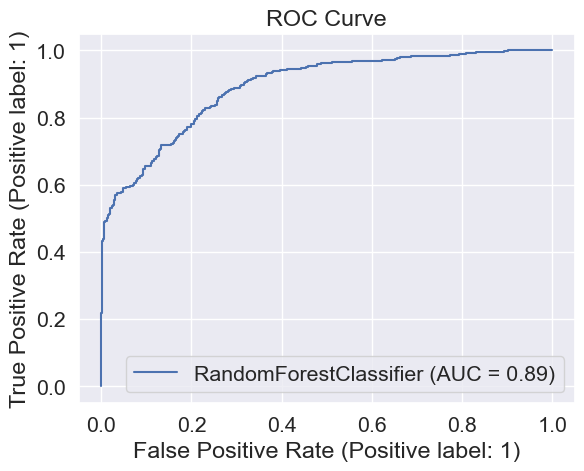
\includegraphics[scale=0.2]{Sec7_19.png}
            }

            \subfigure[Accuracy、Precision、Recall、F1-Score]
            {
                
\includegraphics[scale=0.3]{Sec7_18.png}
            }

            \subfigure[drop部分特征前学习曲线]
            {
                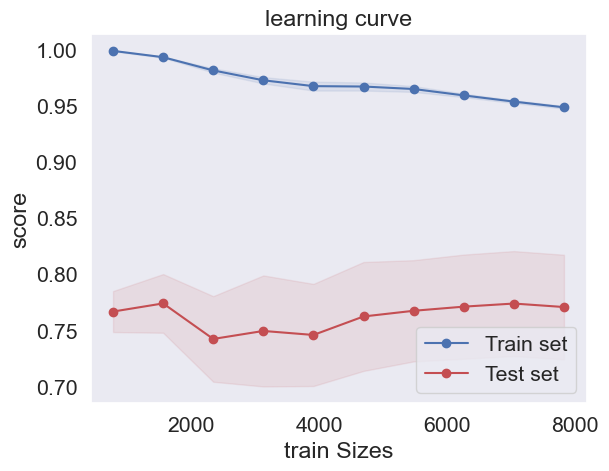
\includegraphics[scale=0.2]{Sec7_20.png}
            }
            \subfigure[drop部分特征后学习曲线]
            {
                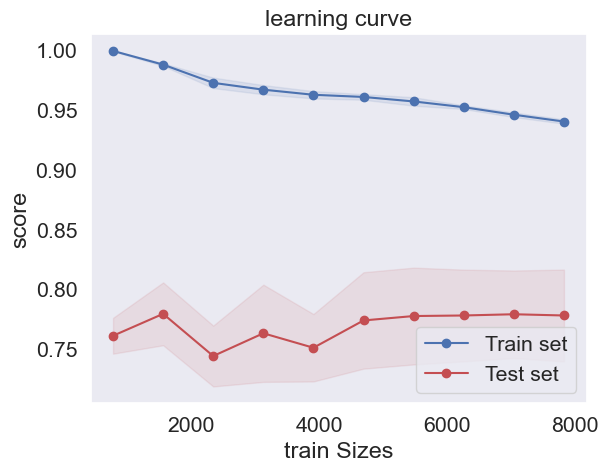
\includegraphics[scale=0.2]{Sec7_28.png}
            }
            \caption{Random Forest}
        \end{figure}

        在Decision Tree中使用的是CART树,而Random Forest的基学习器就是CART决策树,并且具有放回抽样,特征和样本随机采样,无剪枝,投票,可以减小方差的特点。
        由图38.(d)可以发现,此时方差很大,发生了过拟合现象,经过检查是因为数据未进行drop部分特征,drop部分特征后可以发现曲线收敛程度有了很大的改进,并且Random Forst模型的效果相比起Decision Tree有了很大的提升。

    \subsection{CatBoost}

        混淆矩阵如图39.(a)所示,ROC曲线如图39.(b)所示,Accuracy、Precision、Recall、F1-Score如图39.(c)所示,drop部分特征前学习曲线如图39.(d)所示,drop部分特征后学习曲线如图39.(e)所示。

        \begin{figure}[H]
            \centering
            \subfigure[混淆矩阵]
            {
                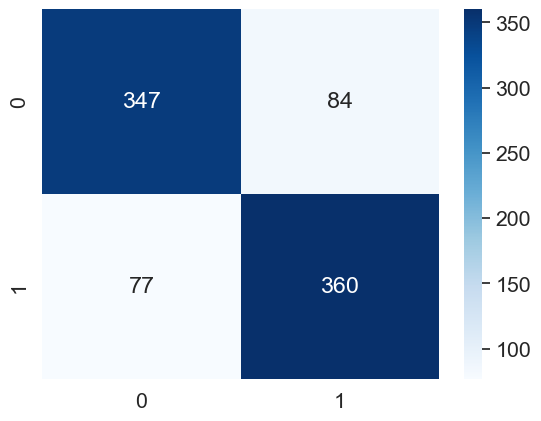
\includegraphics[scale=0.2]{Sec7_21.png}
            }
            \subfigure[ROC曲线]
            {
                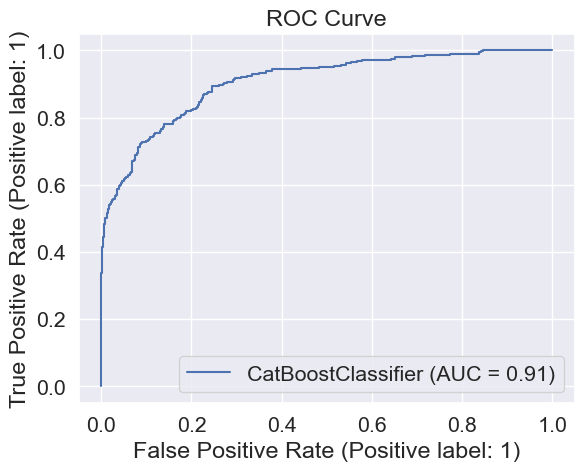
\includegraphics[scale=0.2]{Sec7_23.png}
            }

            \subfigure[Accuracy、Precision、Recall、F1-Score]
            {
                
\includegraphics[scale=0.3]{Sec7_22.png}
            }

            \subfigure[drop部分特征前学习曲线]
            {
                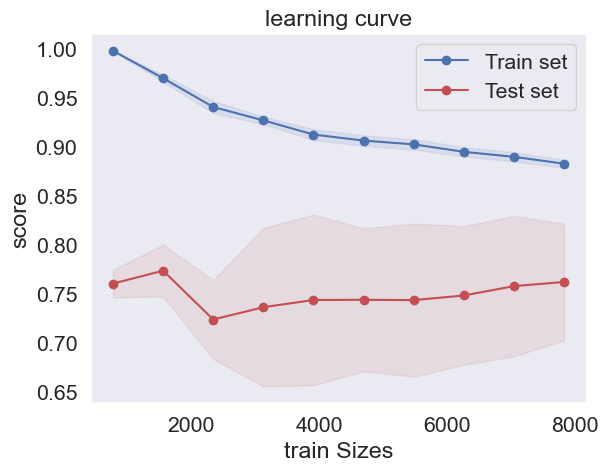
\includegraphics[scale=0.2]{Sec7_24.png}
            }
            \subfigure[drop部分特征后学习曲线]
            {
                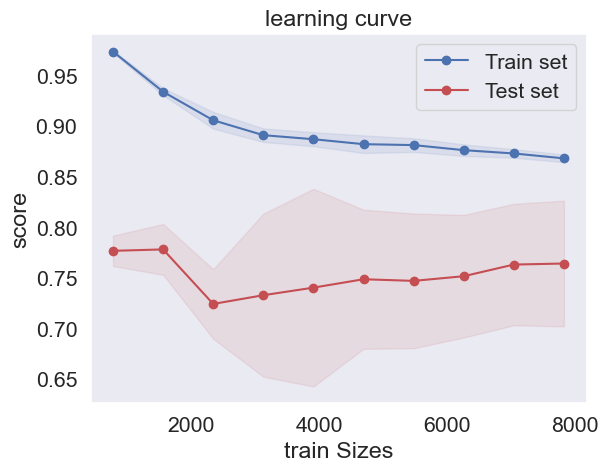
\includegraphics[scale=0.2]{Sec7_29.png}
            }
            \caption{CatBoost}
        \end{figure}

        CatBoost是所有模型中效果最好的,从学习曲线观看可以发现,CatBoost相比起Random Forest大幅度减小了数据的偏差,一定程度上解决了模型欠拟合的问题,使模型效果更好。
        并且从混淆矩阵观看可以发现CatBoost相比起Random Forest加强了对于正类样本的学习能力,同时保证了负类样本的学习能力,因此模型有了更好的效果。

        除此以外,我还尝试了不提前进行编码,直接利用CatBoost的编码功能进行训练,由图40的混淆矩阵和学习曲线所示,可以发现模型效果依然是超越大多数模型,但是没有编码后训练的CatBoost效果好。
        因此编码后的数据更有利于模型的学习。

        \begin{figure}[H]
            \centering
            \subfigure[混淆矩阵]
            {
                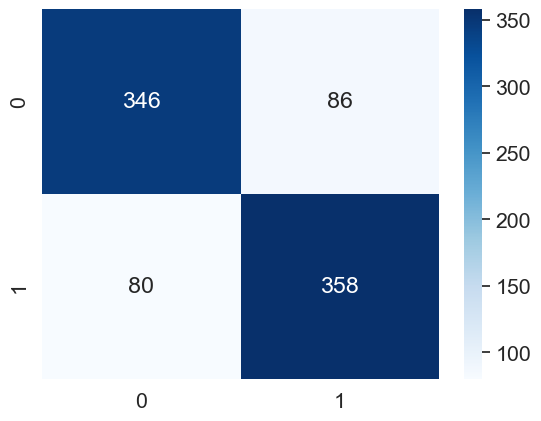
\includegraphics[scale=0.2]{Sec7_31.png}
            }
            \subfigure[学习曲线]
            {
                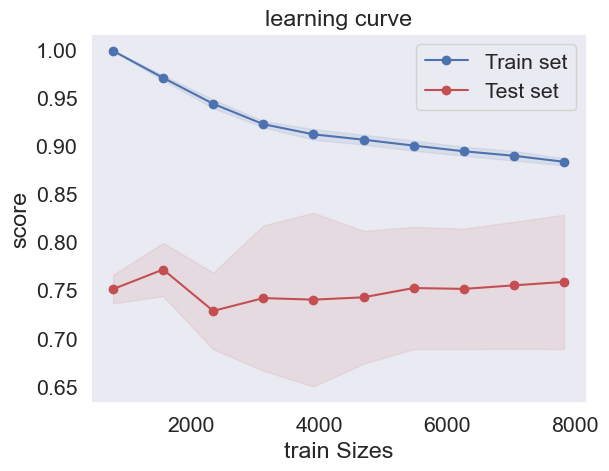
\includegraphics[scale=0.2]{Sec7_32.png}
            }
            \caption{CatBoost}
        \end{figure}

    \subsection{对比}
    
        选择将6个模型的accuracy绘制成柱状图进行对比,如图41所示,并将Accuracy、Precision、Recall、F1-Score、Time五个指标制成表格进行对比,如表7所示。

        \begin{figure}[H]
            \centering
                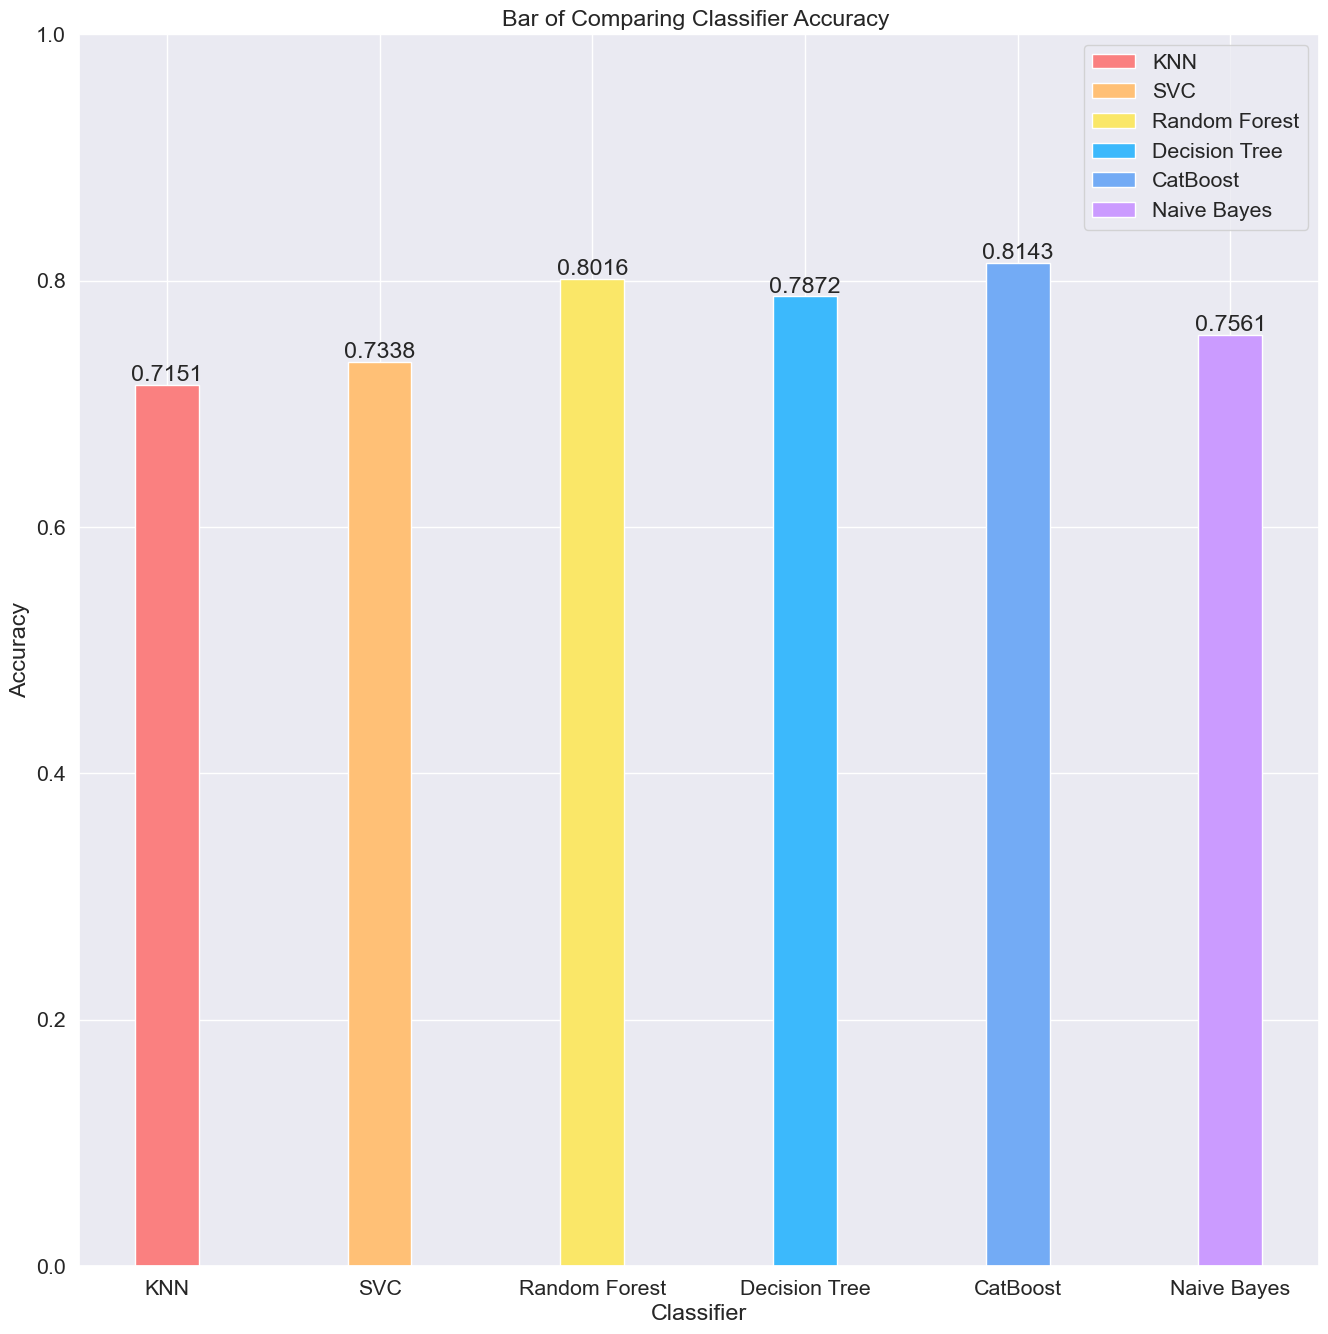
\includegraphics[scale=0.25]{Sec7_33.png}
            \caption{Contrast}
        \end{figure}

        \begin{table}[H]
            \centering
            \footnotesize
            \begin{tabular}{|c|c|c|c|c|c|}
            \hline
            {\color[HTML]{000000} \textbf{Classifier}}    & {\color[HTML]{000000} \textbf{Mean\_Accuracy}} & {\color[HTML]{000000} \textbf{Mean\_Precision}} & {\color[HTML]{000000} \textbf{Mean\_Recal}} & {\color[HTML]{000000} \textbf{Mean\_F1-Score}} & {\color[HTML]{000000} \textbf{Running Time(s)}} \\ \hline
            \rowcolor[HTML]{FFFFFF} 
            {\color[HTML]{000000} \textbf{KNN}}           & {\color[HTML]{000000} 0.7151}                  & {\color[HTML]{000000} 0.741273}                 & {\color[HTML]{000000} 0.667498}             & {\color[HTML]{000000} 0.702177}                & {\color[HTML]{000000} 0.613137}                 \\ \hline
            \rowcolor[HTML]{FFFFFF} 
            {\color[HTML]{000000} \textbf{SVC}}           & {\color[HTML]{000000} 0.7338}                  & {\color[HTML]{000000} 0.778160}                 & {\color[HTML]{000000} 0.659946}             & {\color[HTML]{000000} 0.714015}                & {\color[HTML]{000000} 100.743812}               \\ \hline
            \rowcolor[HTML]{FFFFFF} 
            {\color[HTML]{000000} \textbf{Random Forest}} & {\color[HTML]{000000} 0.8016}                  & {\color[HTML]{000000} 0.814292}                 & {\color[HTML]{000000} 0.786322}             & {\color[HTML]{000000} 0.799697}                & {\color[HTML]{000000} 16.315396}                \\ \hline
            \rowcolor[HTML]{FFFFFF} 
            {\color[HTML]{000000} \textbf{Decision Tree}} & {\color[HTML]{000000} 0.7872}                  & {\color[HTML]{000000} 0.788545}                 & {\color[HTML]{000000} 0.790662}             & {\color[HTML]{000000} 0.788867}                & {\color[HTML]{000000} 0.307016}                 \\ \hline
            \rowcolor[HTML]{FFFFFF} 
            {\color[HTML]{000000} \textbf{CatBoost}}      & {\color[HTML]{000000} 0.8143}                  & {\color[HTML]{000000} 0.811169}                 & {\color[HTML]{000000} 0.823589}             & {\color[HTML]{000000} 0.817136}                & {\color[HTML]{000000} 12.059265}                \\ \hline
            \rowcolor[HTML]{FFFFFF} 
            {\color[HTML]{000000} \textbf{Naive Bayes}}   & {\color[HTML]{000000} 0.7561}                  & {\color[HTML]{000000} 0.777445}                 & {\color[HTML]{000000} 0.723057}             & {\color[HTML]{000000} 0.749048}                & {\color[HTML]{000000} 0.091428}                 \\ \hline
            \end{tabular}
            \caption{模型指标对比}
        \end{table}

        可以发现,CatBoost可以在相对较少的训练时间的情况下,取得超越其他模型的效果,符合预期。

        除此以外,我们还对测试集进行了预测,并将预测结果提交到Kaggle上进行测试,计算得分,如表8所示。

        \begin{table}[H]
            \footnotesize
            \centering
            \begin{tabular}{|c|c|}
            \hline
            \textbf{Model} & \textbf{Score} \\ \hline
            SVC            & 0.74959        \\ \hline
            Decision Tree  & 0.77764        \\ \hline
            Naive Bayes    & 0.76408        \\ \hline
            KNN            & 0.72013        \\ \hline
            Random Forest  & 0.79237        \\ \hline
            CatBoost       & 0.80313        \\ \hline
            \end{tabular}
        \end{table}

        可以看到虽然分数与交叉验证的结果有差别,但是模型效果的好坏相对是一致的。

\end{document}